\subsection{Estación de servicio}
\subsubsection{Descripción del experimento}
El experimento se realizó en una estación de servicio, en la cual se ejecutó el programa de captura de paquetes ARP durante aproximadamente $46$ minutos. Los resultados y el análisis de los mismos se encuentran abajo.

\subsubsection{Resultados del experimento}

\begin{landscape}
\begin{figure}[H]
  \centering	
	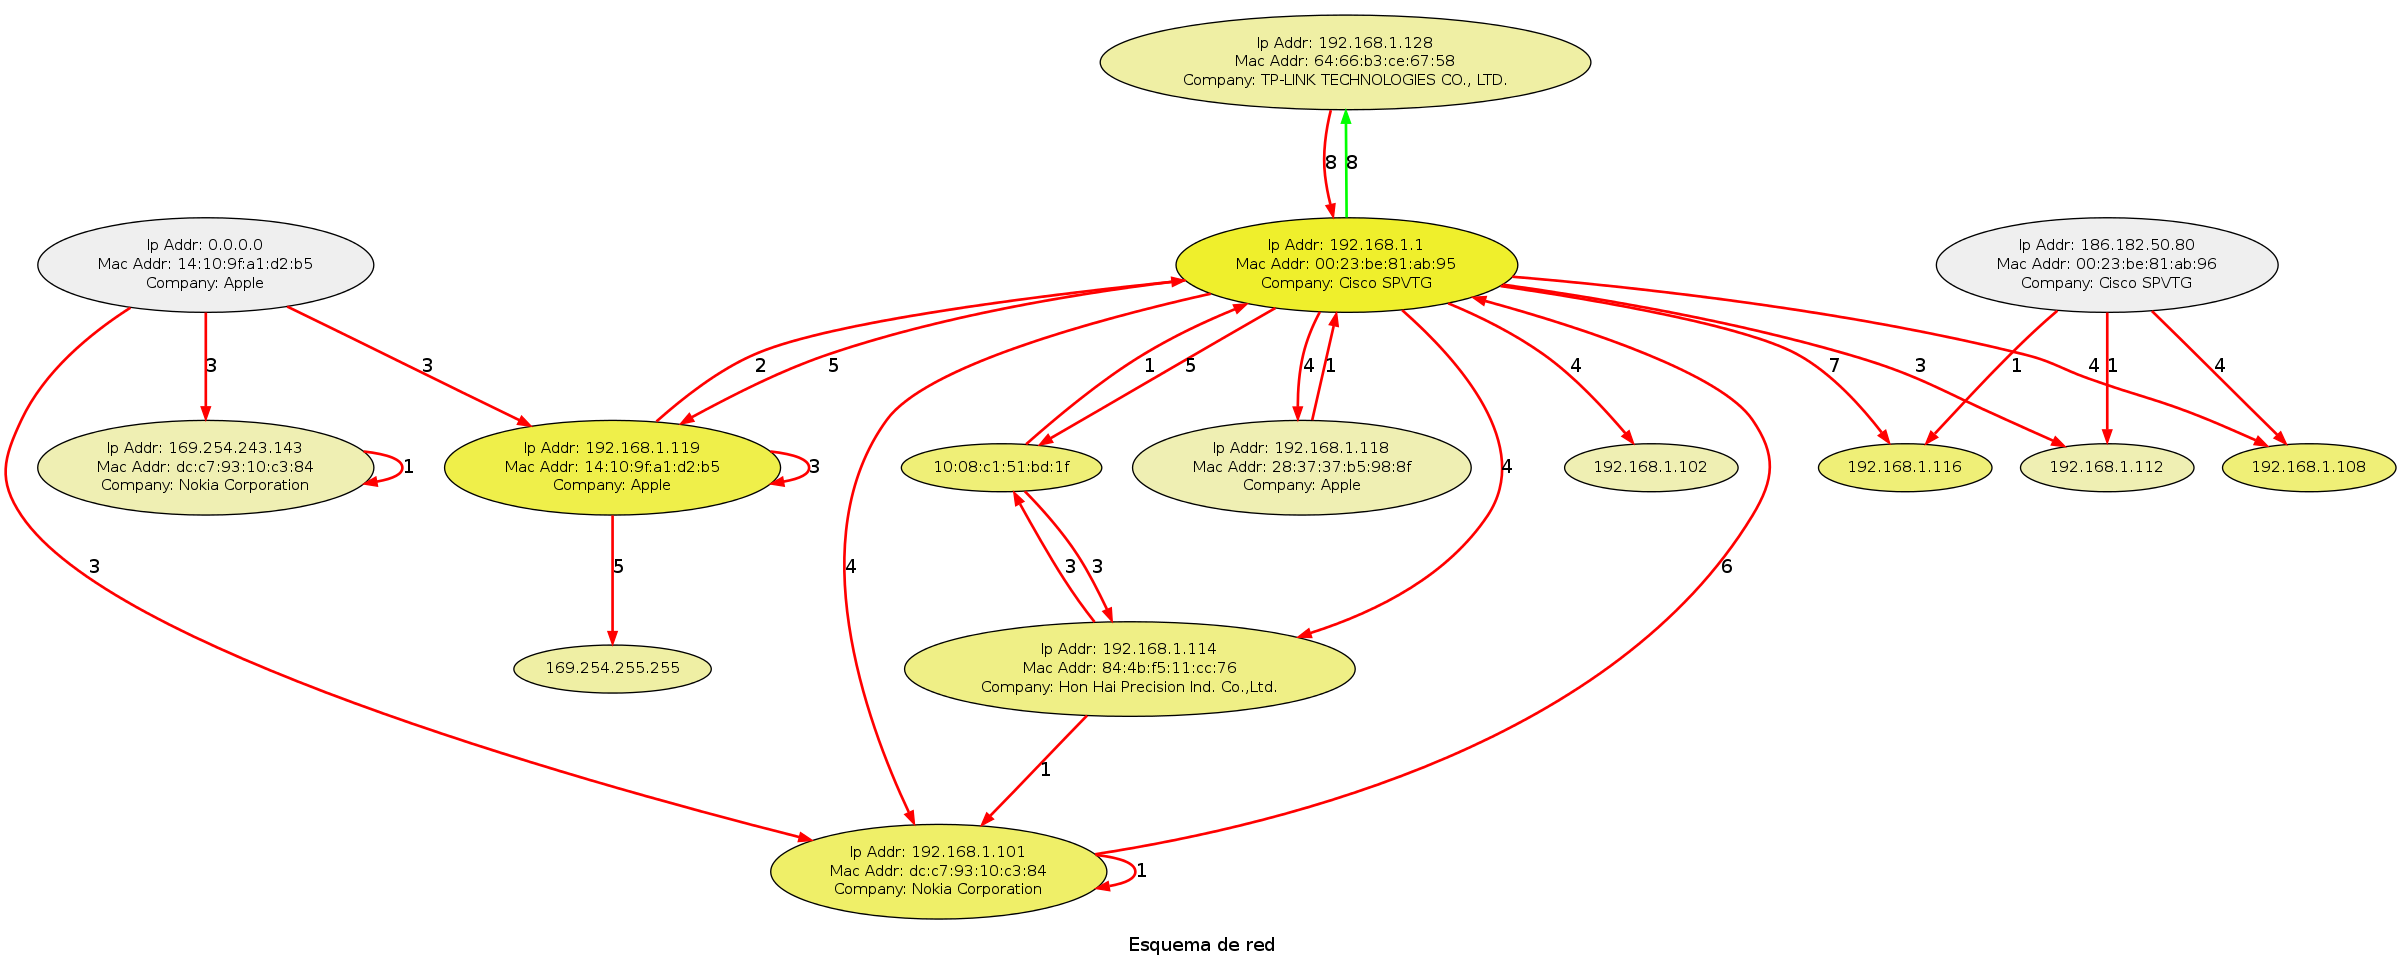
\includegraphics[scale=0.30]{../experimentacion-barbeiton/graph.png}
  \caption{Grafo de la red analizada según los paquetes ARP.}
\end{figure}
\end{landscape}

\begin{figure}[H]
  \centering	
	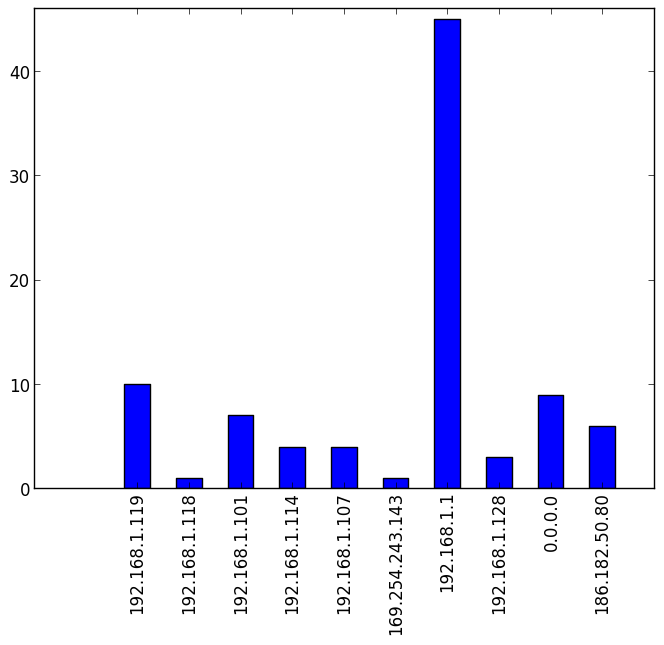
\includegraphics[scale=0.66]{../experimentacion-barbeiton/histogram_src.png}
  \caption{Histograma de las IP fuente.}
\end{figure}

\begin{figure}[H]
  \centering
	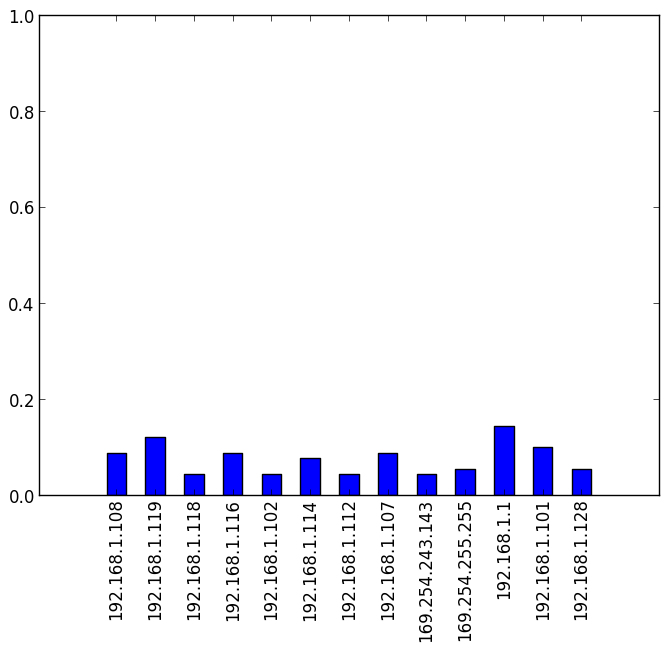
\includegraphics[scale=0.66]{../experimentacion-barbeiton/histogram_dst_probabilities.png}
  \caption{Probabilidades asociadas a las IP de la fuente destino.}
\end{figure}

\begin{figure}[H]
  \centering	
	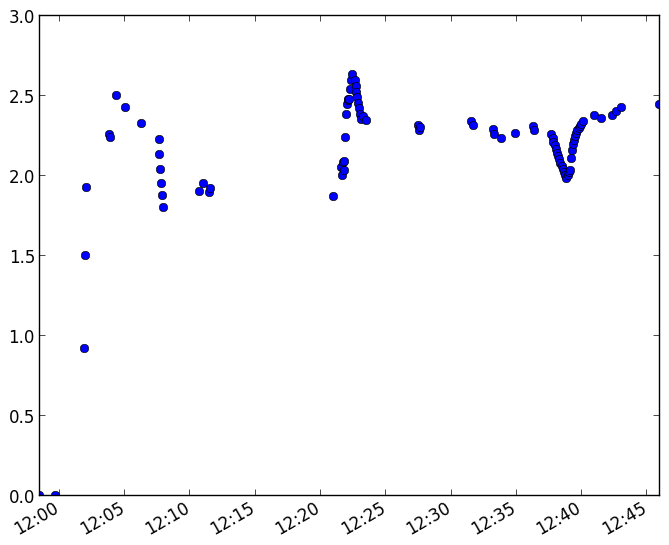
\includegraphics[scale=0.66]{../experimentacion-barbeiton/entropy_src.png}
  \caption{Entropía en función del tiempo tomando como fuente las IP source.}
\end{figure}

\begin{figure}[H]
  \centering
	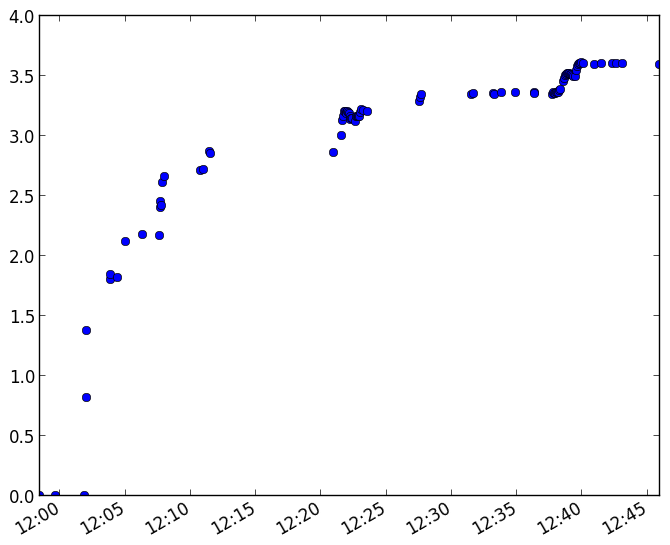
\includegraphics[scale=0.66]{../experimentacion-barbeiton/entropy_dst.png}
  \caption{Entropia de la fuente de IP destino.}
\end{figure}

\subsubsection{Conclusiones del experimento}
En la Figura $15$ podemos ver el grafo de la red según el intercambio de paquetes ARP. Se puede notar que el nodo que intercambia la mayor cantidad de paquetes ARP es el de IP número 192.168.1.1. El dispositivo con dicha IP parece estar al centro del intercambio de los paquetes ARP en la red, con lo que podemos concluir que se trata de un access point. El hecho de que este dispositivo tenga ese número de IP es una evidencia en favor de esa suposición, ya que es una dirección usual para access points.
\par Durante la hora en la cual se realizó el experimento, podemos ver que la entropía de la fuente $S_{src}$ fue variando considerablemente, aunque siempre tiende al aumento, como puede verse en la figura $16$. La entropía de la fuente de información modelada como $S_{dst}$ también tiende a aumentar, aunque de forma mucho menos errática que la anterior. 
\par En la figura $14$ podemos ver que nuevamente, el nodo con IP 192.168.1.1 se destaca con respecto a los demás. En este gráfico se muestra que la cantidad de paquetes que ARP que envía este nodo es más de $4$ veces superior a los demás nodos. 
\par Un dato interesante que surge de la figura $14$ es la aparición de la IP 0.0.0.0. Esta IP es una dirección que podría aparecer en un host cuando éste no tiene aignada una dirección de IP válida.

